
\begin{TP}[Plusieurs symétries de suite \ldots]

Que se passe‑t‑il lorsqu'on fait subir à une figure plusieurs symétries axiales, l'une à la suite de l'autre ? \\[0.5em]
Par exemple, on construit d'abord le symétrique d'une figure par rapport à un axe $d$. On obtient une nouvelle figure, et on construit le symétrique de cette nouvelle figure par rapport à une autre droite $d'$. \\[0.5em]
Pour répondre à cette question, répartissez votre groupe en deux sous‑groupes. Le premier travaillera avec papier, crayon et instruments de géométrie. L'autre utilisera un logiciel de géométrie dynamique comme TracenPoche. \\[0.5em]
L'objectif de ce travail est de pouvoir répondre plus précisément aux questions suivantes.
\begin{enumerate}
 \item Que se passe‑t‑il si $d$ et $d'$ sont parallèles ?
 \item Que se passe‑t‑il si $d$ et $d'$ sont sécantes et non perpendiculaires en un point $O$ ?
 \item Que se passe‑t‑il si $d$ et $d'$ sont perpendiculaires ?
 \end{enumerate}
\begin{center} 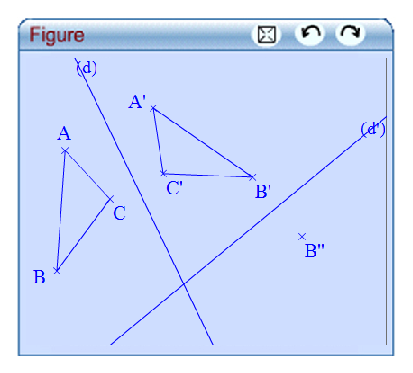
\includegraphics[width=6.7cm]{TracenPoche} \end{center}
\end{TP}

%%%%%%%%%%%%%%%%%%%%%%%%%%%%%%%%%%%%%%%%%%%%%%%%%%%%%%%%%%%%%%%%%%%%%%

\begin{TP}[Pavage rectangulaire]

Un pavage est une méthode de remplissage d'un espace à l'aide d'un motif répétitif, sans trou ni débordement.

\partie{Un pavage imposé}
\begin{enumerate}
\begin{minipage}[c]{0.58\linewidth}
 \item À partir d'une feuille au format A4, effectuez deux pliages pour obtenir quatre rectangles de même taille comme sur le schéma ci-contre.
 \end{minipage} \hfill%
 \begin{minipage}[c]{0.38\linewidth}
 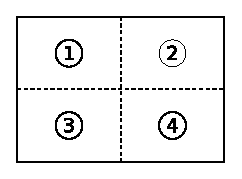
\includegraphics[width=3.7cm]{pavage1234}
  \end{minipage} \\
 \item Sur votre feuille, construisez dans le rectangle \circled{1}, la figure ci-dessous ($O$ est le centre de l'arc de cercle) : ($AD = DO$ et $BI = IC$)
 \begin{center} 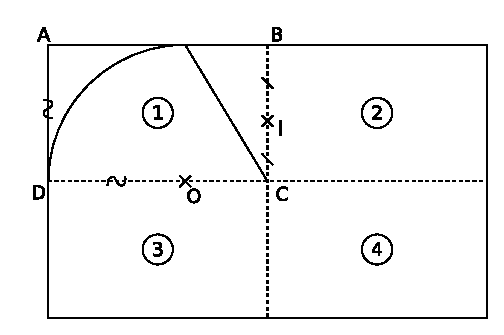
\includegraphics[width=8.2cm]{pavageABCD} \end{center}
 \item Construisez le symétrique par rapport à $I$ de la figure tracée dans le rectangle \circled{1}. Dans quelle partie de la feuille va-t-il se situer ?
 \item Construisez les symétriques par rapport à la droite $(DC)$ des figures des parties \circled{1} et \circled{2}.
 \end{enumerate}
Rassemblez toutes les feuilles du groupe que vous placerez les unes à côté des autres pour former un grand rectangle. C'est un pavage rectangulaire.

\partie{Un pavage libre}
À partir de nouvelles feuilles A4, tracez, dans le rectangle  \circled{1}, un motif géométrique composé de droites, segments ou cercles. Tous les élèves du groupe doivent avoir exactement le même motif. \\[0.5em]
De la même façon qu'auparavant construisez l'image, par la symétrie de centre $I$, de la figure tracée dans le rectangle \circled{1} puis l'image, par la symétrie d'axe $(DC)$, des figures tracées dans les rectangles \circled{1} et \circled{2}. \\[0.5em]
En regroupant les feuilles, on obtient ainsi un nouveau pavage rectangulaire.
\end{TP}

